%
% datenblaetter.tex -- Anhang mit einer Zusammenstellung aller Datenblaetter
%
% (c) 2015 Prof Dr Andreas Mueller, Hochschule Rapperswil
%
\chapter{Verteilungs-Datenblätter} \label{chapter:datenblaetter}
Die folgenden Abschnitte stellen die wichtigsten Eigenschaften der
verschiedenen in früheren Kapiteln behandelten Verteilungen zusammen.

\section{Gleichverteilung}
%
% db-gleichverteilung.tex -- Datenblatt der stetigen gleichverteilung
%
% (c) 2015 Prof Dr Andreas Mueller, Hochschule Rapperswil
%
\subsection{Steckbrief}
\begin{center}
\begin{tabular}{|l|l|}
\hline
Name&Gleichverteilung\\
\hline
Dichtefunktion&
\begin{minipage}{3.7in}
\vskip5pt
$\displaystyle
\begin{cases}
\frac1{b-a}&\qquad a\le x\le b\\
0&\qquad\text{sonst}
\end{cases}
$
\end{minipage}
\\[8pt]
Verteilungsfunktion&
\begin{minipage}{3.7in}
\vskip5pt
$\displaystyle
\begin{cases}0&\qquad x\le a\\
\frac{x-a}{b-a}&\qquad x \le a \le b\\
1&\qquad x>b\end{cases}
$
\end{minipage}
\\[8pt]
Erwartungswert&
\begin{minipage}{3.7in}
\vskip3pt
$\displaystyle \frac{a+b}2$
\end{minipage}
\\[8pt]
Varianz&
\begin{minipage}{3.7in}
\vskip3pt
$\displaystyle \frac{(b-a)^2}{12}$
\end{minipage}
\\[8pt]
Median&
\begin{minipage}{3.7in}
\vskip3pt
$\displaystyle \frac{a+b}{2}$
\end{minipage}
\\[8pt]
$P(|X-E(X)|>\varepsilon)$&
\begin{minipage}{3.7in}
\vskip3pt
$\displaystyle 1-\frac{2\varepsilon}{b-a}$ für $\varepsilon<\frac{b-a}2$
\end{minipage}
\\[10pt]
\hline
Anwendungen&\begin{minipage}{3.7in}%
\strut
$\bullet$ Verteilung von Zufallszahlen
\strut
\end{minipage}\\
\hline
\end{tabular}
\end{center}

\subsection{Verteilungsfunktion und Wahrscheinlichkeitsdichte}
Verteilungsfunktion (oben) und Wahrscheinlichkeitsdichte (unten)
der Gleichverteilung:
\begin{center}
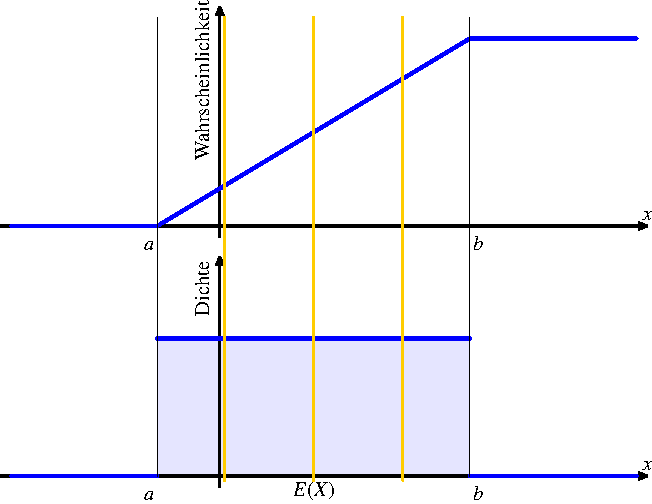
\includegraphics[width=0.8\hsize]{images/verteilungsfunktion-7}
\end{center}

\subsection{Wahrscheinlichkeit einer grossen Abweichung}
Wahrscheinlichkeit einer Abweichung vom Mittelwert einer
in $[0,1]$ gleichverteilten Zufallsvariable (rot) im Vergleich mit
der oberen Schranke aus dem Satz von Tschebyscheff (grün):
\begin{center}
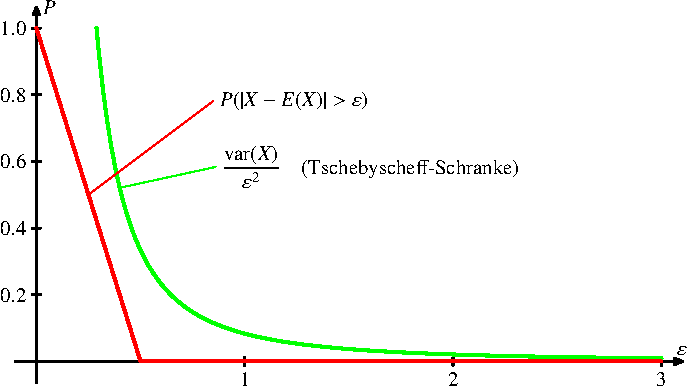
\includegraphics{images/gl-1.pdf}
\end{center}

\subsection{Parameter schätzen}
Die Parameter $a$ und $b$ der Gleichverteilung können mit den 
erwartungstreuen Schätzern
\begin{align*}
\hat a(x_1,\dots,x_n)=\frac{n+1}{n}\min(x_1,\dots,x_n)\\
\hat b(x_1,\dots,x_n)=\frac{n+1}{n}\max(x_1,\dots,x_n)
\end{align*}
geschätzt werden.

\vfill
\pagebreak

\section{Exponentialverteilung}
%
% db-exponentialverteilung.tex -- Datenblatt der Exponentialverteilung
%
% (c) 2015 Prof Dr Andreas Mueller, Hochschule Rapperswil
%
\subsection{Steckbrief}
\begin{center}
\renewcommand{\arraystretch}{2}
\begin{tabular}{|l|l|}
\hline
Name&Exponentialverteilung\\
\hline
Dichtefunktion&$\displaystyle ae^{-ax}$\\
Verteilungsfunktion&$1-e^{-ax}$\\
Erwartungswert&$\displaystyle \frac1a$\\
Varianz&$\displaystyle \frac1{a^2}$\\
Median&$\displaystyle \frac1a\log 2$\\[8pt]
$P(|X-E(X)|>\varepsilon)$&
\begin{minipage}{3.7in}
$
\begin{cases}
e^{-a\varepsilon-1}&\qquad\text{f"ur $\varepsilon > \frac1a$}\\
1-e^{a\varepsilon-1}+e^{-a\varepsilon-1}&\qquad\text{f"ur $\varepsilon \le \frac1a$}
\end{cases}
$
\end{minipage}
\\[10pt]
\hline
Anwendungen&\begin{minipage}{3.7in}%
\strut
$\bullet$ Prozess ohne Erinnerungsverm"ogen\\
$\bullet$ Radioaktivit"at
\strut
\end{minipage}\\
\hline
\end{tabular}
\end{center}

\subsection{Verteilungsfunktion und Wahrscheinlichkeitsdichte}
Verteilungsfunktion (oben) und Dichtefunktion (unten) der
Exponentialverteilung:
\begin{center}
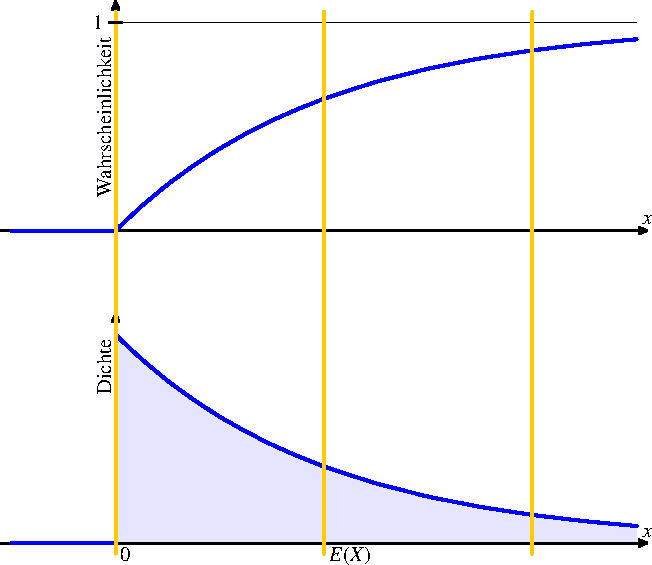
\includegraphics[width=0.8\hsize]{images/verteilungsfunktion-8}
\end{center}

\subsection{Wahrscheinlichkeit grosser Abweichungen}
Wahrscheinlichkeit f"ur eine grosse Abweichung bei einer
Exponentialverteilten Zufallsvariable, oben die durch den Satz von Tschebyscheff
gegebene Schranke (gr"un), unten die exakte Rechnung mit
Hilfe der Exponentialvereteilung (rot):
\begin{center}
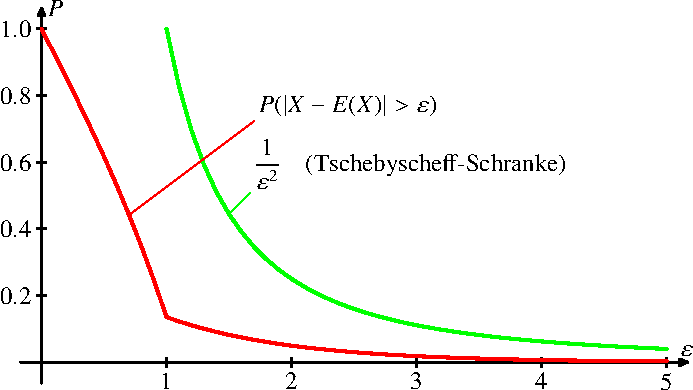
\includegraphics{images/exp-1.pdf}
\end{center}

\subsection{Parameter sch"atzen}
Der Parameter $1/a$ kann mit dem erwartungstreuen Sch"atzer
\[
\frac1{\hat a(x_1,\dots,x_n)}=\frac{x_1+\dots+x_n}n
\]
gesch"atzt werden.

\subsection{Erlang-Verteilungen}
Sie $X_i$ unabh"angige, identisch mit Parameter $a$ exponentialverteilte
Zufallsvariablen.
Dann ist $X_1+\dots+X_n$ Erlang-verteilt. 
Die Erlang-Verteilungen wurden f"ur die Analyse von Telefonzentralen erfunden,
und sind allgemein in der Queueing-Theorie n"utzlich.
Die Wahrscheinlichkeitsdichte und die Verteilungsfunktionen sind
\begin{align*}
F_{X_1+\dots+X_k}(x)&=\begin{cases}
\displaystyle 1-e^{-ax}\sum_{i=0}^{k-1}\frac{(ax)^i}{i!}&\qquad x\ge 0\\
\displaystyle 0&\qquad x < 0
\end{cases}
\\
\varphi_{X_1+\dots+X_k}(x)&=\begin{cases}
\displaystyle a^k\frac{x^{k-1}}{(k-1)!}e^{-ax}&\qquad x\ge 0\\
\displaystyle 0&\qquad x<0.
\end{cases}
\end{align*}

\vfill
\pagebreak

\section{Normalverteilung}
%
% db-normalverteilung.tex -- datenblatt der Normalverteilung
%
% (c) 2015 Prof Dr Andreas Mueller, Hochschule Rapperswil
%
\subsection{Steckbrief}
\begin{center}
\renewcommand{\arraystretch}{2}
\begin{tabular}{|l|l|}
\hline
Name&Normalverteilung\\
\hline
\setlength{\extrarowheight}{2pt}
Dichtefunktion&$\displaystyle\frac{1}{\sqrt{2\pi}\sigma}e^{-\frac{(x-\mu)^2}{2\sigma^2}}$\\
Verteilungsfunktion&keine elementare Funktion\\
Erwartungswert&$\mu$\\
Varianz&$\sigma^2$\\
Median&$\mu$\\
$P(|X-E(X)|>\varepsilon)$&keine einfache Formel\\
\hline
%\setlength{\extrarowheight}{50pt}
Anwendungen&
\begin{minipage}{3.7in}%
\vskip4pt
\strut
$\bullet$ Messwerte\\
$\bullet$ Summe vieler kleiner Einflüsse vergleichbar grosser Varianz
(Zentraler Grenzwertsatz)
\\
$\bullet$ Approximation der Binomialverteilung
\strut
\end{minipage}\\[21pt]
\hline
\end{tabular}
\end{center}

\subsection{Verteilungsfunktion und Wahrscheinlichkeitsdichte}
Verteilungsfunktion (oben) und Dichtefunktion (unten) der Normalverteilung:
\begin{center}
%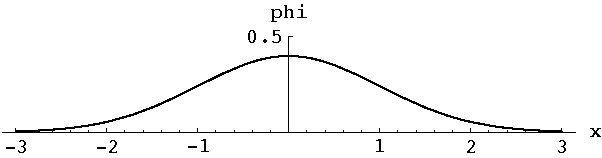
\includegraphics[width=0.8\hsize]{graphics/normphi}
%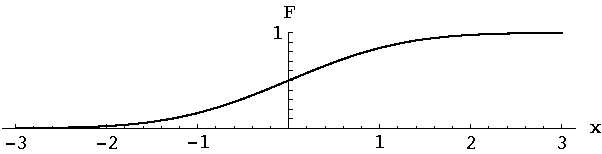
\includegraphics[width=0.8\hsize]{graphics/normF}
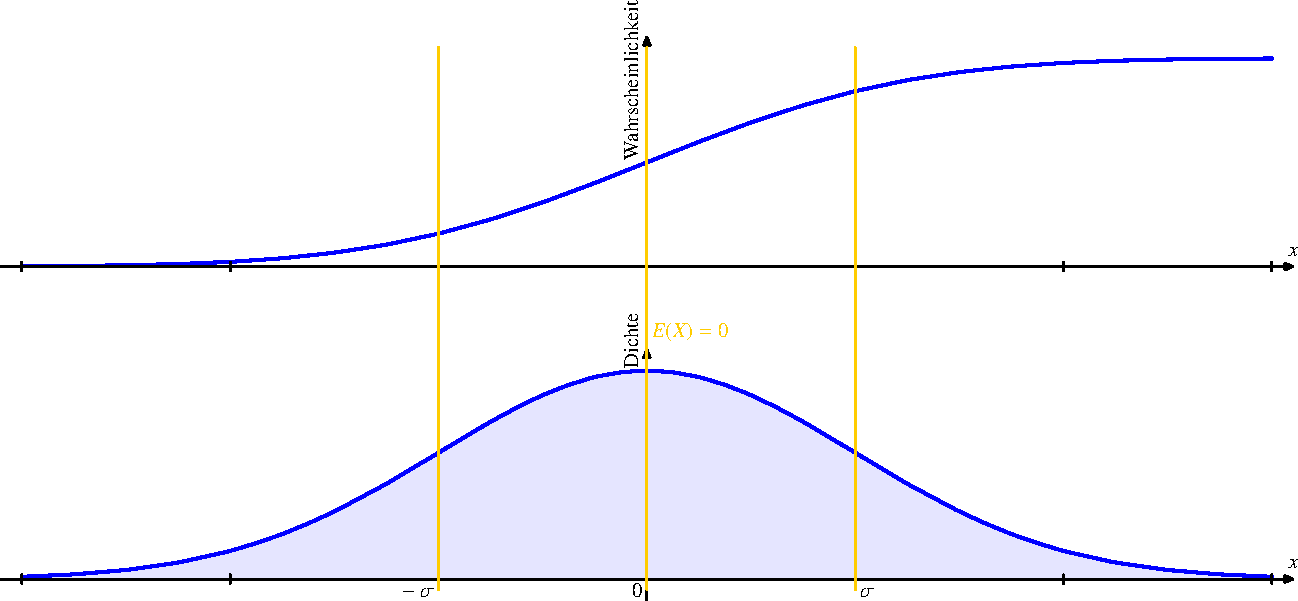
\includegraphics[width=\hsize]{images/verteilungsfunktion-9}
\end{center}

\subsection{Wahrscheinlichkeit einer grossen Abweichung}
Vergleich der Wahrscheinlichkeit für eine grosse Abweichung
für die Normalverteilung (rot) und die Schranke von Tschebyscheff (grün):
\begin{center}
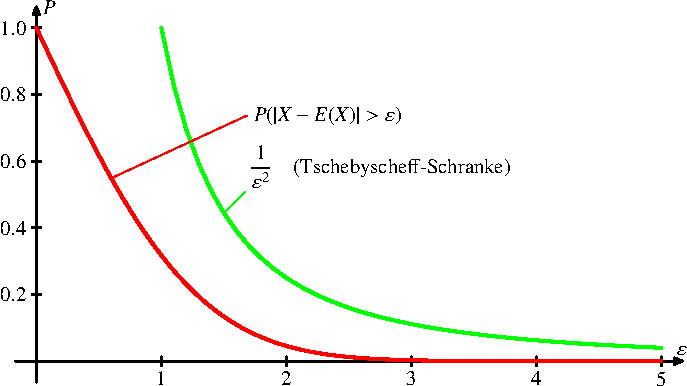
\includegraphics{images/norm-1.pdf}
\end{center}

\subsection{Parameter schätzen}
Die Parameter $\mu$ und $\sigma$ können mit den erwartungstreuen Schätzern
\begin{align*}
\hat\mu(x_1,\dots,x_n)&=\frac{x_1+\dots+x_n}{n}\\
\hat\sigma(x_1,\dots,x_n)^2&=\frac{1}{n-1}\biggl(
\sum_{i=1}^n x_i^2 - \frac1n\biggl(\sum_{i=1}^n x_i\biggr)^2
\biggr)
\end{align*}
geschätzt werden.

Der Mittelwert ist $\hat\mu(x_1,\dots,x_n)$ ist normalverteilt mit Erwartungswert
$\mu$ und Varianz $\frac1n\sigma^2$.
Die Stichprobenvarianz $\hat\sigma(x_1,\dots,x_n)^2/\sigma^2$ ist $\chi^2$-verteilt
mit $n-1$ Freiheitsgraden.

\subsection{Zentraler Grenzwertsatz}
Der zentrale Grenzwertsatz besagt, dass die Verteilungsfunktion einer Summe
einer grossen Zahl von Zufallsvariablen unter milden Voraussetzungen
gegen die Verteilungsfunktion einer Normalverteilung konvergiert.
Dies rechtfertigt den Einsatz der Normalverteilung als Modell für Prozesse,
in denen eine grosse Zahl von vergleichbar grossen Einflüssen zu einem Effekt
beitragen, zum Beispiel bei Messwerten.

\subsection{Standardisierung}
Ist $X$ eine normalverteilte Zufallsvariable, dann ist 
\[
Z=\frac{X-\mu}{\sigma}
\]
eine normalverteilte Zufallsvariable mit Erwartungswert $0$ und Varianz $1$,
d.~h.~eine standardnormalverteilte Zufallsvariable.
Für die Standardnormalverteilung ist im Tabellenanhang eine Tabelle der
Verteilungsfunktion sowie einzelner Quantilen zu finden.

Man beachte, dass die Zufallsvariable $Z$ nicht mehr normalverteilt ist, wenn man
$\mu$ und $\sigma$ durch Schätzwerte ersetzt, die resultierende Verteilung
ist dann eine $t$-Verteilung.

\vfill
\pagebreak

\section{Potenzgesetz, Pareto-Verteilung}
%
% db-paretoverteilung.tex -- Datenblatt der Pareto-Verteilung
%
% (c) 2015 Prof Dr Andreas Mueller, Hochschule Rapperswil
%
\subsection{Steckbrief}
\begin{center}
\renewcommand{\arraystretch}{2}
\begin{tabular}{|l|l|}
\hline
Name&Potenzverteilung, Pareto-Verteilung\\
\hline
Dichtefunktion&
\begin{minipage}{3.7in}
\vskip5pt
$\displaystyle
\begin{cases}
\frac{\alpha-1}{x_{\min}}\biggl(\frac{x}{x_{\text{min}}}\biggr)^{-\alpha}&\qquad x>x_{\text{min}}\\
0&\qquad\text{sonst}
\end{cases}
$
\end{minipage}
\\[15pt]
Verteilungsfunktion&
\begin{minipage}{3.7in}
\vskip3pt
$\displaystyle
\begin{cases}
1-\biggl(\frac{x}{x_{\text{min}}}\biggr)^{1-\alpha}&\qquad x>x_{\text{min}}\\
0&\qquad\text{sonst}
\end{cases} $
\end{minipage}
\\
Erwartungswert&$\displaystyle\frac{\alpha-1}{\alpha-2}x_{\text{min}}$,
undefiniert f"ur $\alpha\le 2$\\
Varianz&$\displaystyle
\biggl(
\frac{\alpha-1}{\alpha -3}-\biggl(\frac{\alpha-1}{\alpha-2}\biggr)^2
\biggr)x_{\text{min}}^2$, undefiniert f"ur $\alpha \le 3$\\
$P(|X-E(X)|>\varepsilon)$&$\displaystyle $ \\
Median&$2^{\frac1{\alpha-1}}x_{\text{min}}$\\
\hline
Anwendungen&\begin{minipage}{3.7in}%
\vskip5pt
\strut
$\bullet$ H"aufkeitsverteilung f"ur skaleninvariante Prozesse\\
$\bullet$ Einkommensverteilung\\
$\bullet$ Gr"osse und H"aufigkeit von Mondkratern\\
$\bullet$ Verkaufszahlen von B"uchern\\
$\bullet$ Einwohnerzahlen von St"adten
\strut
\end{minipage}\\[28pt]
\hline
\end{tabular}
\end{center}

\subsection{Wahrscheinlichkeitsdichte}
Wahrscheinlichkeitsdichte einer Potenzverteilung mit $\alpha=2.5$,
diese Verteilung hat keine Varianz:
\begin{center}
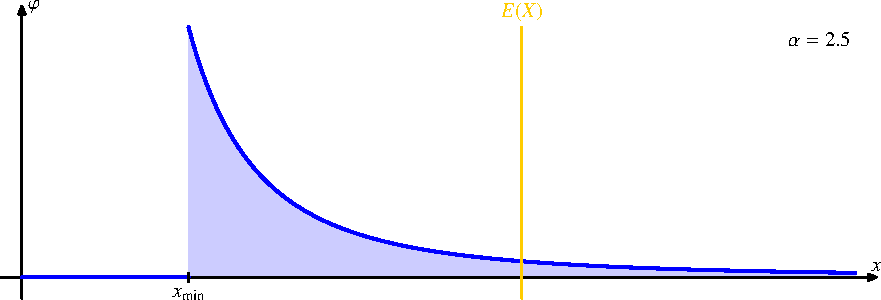
\includegraphics{images/power-2.pdf}
\end{center}

Wahrscheinlichkeitsdichte einer Potenzverteilung mit $\alpha=3.5$:
\begin{center}
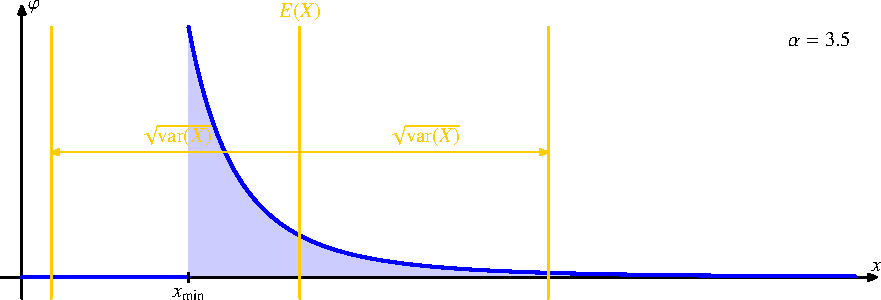
\includegraphics{images/power-3.pdf}
\end{center}

\subsection{80/20-Regeln}
Potenzgesetze geben Anlass zu 80/20-Regeln.
Wir bezeichnen die Wahrscheinlichkeit des Auftretens von Werten $x>0$ 
mit $P(x)=1-F(x)$ und den Anteil des Erwartungswertes dieser Wert
am gesamten Erwartungswert  mit
\[
W(x)=\frac{\int_x^\infty \xi\varphi(\xi)\,d\xi}{\int_{x_{\text{min}}}^\infty \xi\varphi(\xi)\,d\xi}.
\]
Man kann $W(x)$ als den Anteil des ``Wertes'' interpretieren,
den die Werte oberhalb von $x$ beisteuern.
Es ist klar, dass $P(x)=1$ auch bedeutet, $W(x)=1$: 100\% der Werte
tragen 100\% des Wertes bei.
Die Definitionen besagen, dass f"ur beliebiges $x$ der obere $P(x)$-Anteil
der Werte den Anteil $W(x)$ des gesamten Wertes beitragen.
Es gilt
\[
W(x)= P(x)^{\frac{\alpha-2}{\alpha-1}}.
\]
Kurven $(P(x),W(x))$ f"ur verschiedene Werte von $\alpha$:
\begin{center}
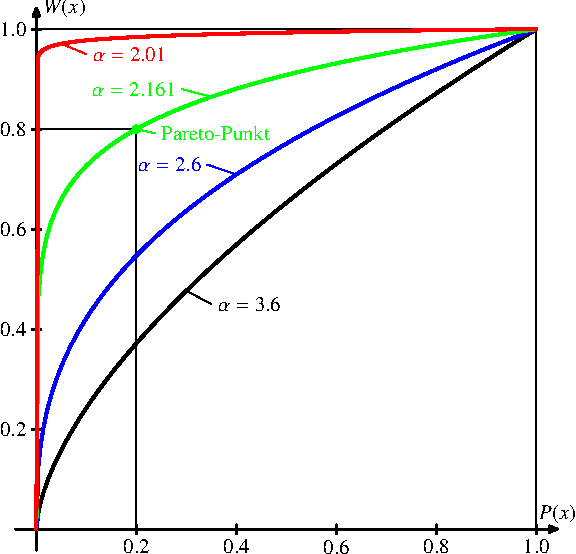
\includegraphics{images/power-4.pdf}
\end{center}


\vfill
\pagebreak

\section{Binomialverteilung}
%
% db-binomialverteilung.tex -- Datenblatt der Binomialverteilung
%
% (c) 2015 Prof Dr Andreas Mueller, Hochschule Rapperswil
%
\subsection{Steckbrief}
\begin{center}
\renewcommand{\arraystretch}{1.5}
\begin{tabular}{|l|l|}
\hline
Name&Binomialverteilung\\
\hline
Wahrscheinlichkeit&
\begin{minipage}{3.7in}
\vskip3pt
$\displaystyle P(k)=\binom{n}{k}p^k(1-p)^{n-k}$
\end{minipage}
\\[10pt]
Verteilungsfunktion&
$\displaystyle F(k)=\sum_{i=0}^k\binom{n}{i}p^i(1-p)^{n-i}$
\\[10pt]
Erwartungswert&$\displaystyle np$\\
Varianz&$\displaystyle np(1-p)$\\
\hline
Anwendungen&\begin{minipage}{3.7in}%
\strut
$\bullet$ Anzahl Eintreten eines Bernoulli-Experimentes
\strut
\end{minipage}\\
\hline
\end{tabular}
\end{center}

\subsection{Verteilungsfunktion und Wahrscheinlichkeitsverteilung}
Wahrscheinlichkeitsverteilung und Verteilungsfunktion einer
Binomialverteilung mit $p=0.4$ und $n=10$:
\begin{center}
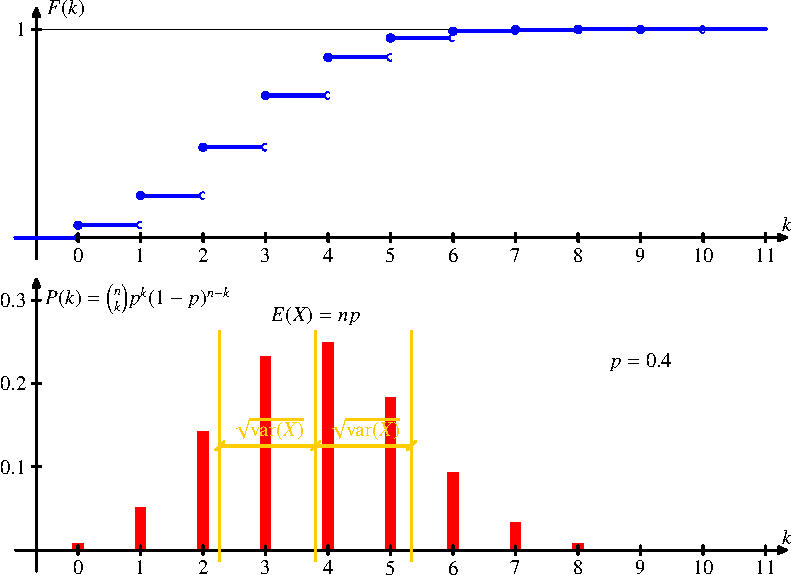
\includegraphics{images/gl-3.pdf}
\end{center}

\subsection{Parameter sch"atzen}
Wir ein Bernoulli-Experiment mit $m$ Wiederholungen $n$ mal wiederholt, erh"alt
man $n$ Werte $k_1,\dots,k_n$.
Die Wahrscheinlichkeit $p$ kann daraus mit Hilfe des Mittelwertes erwartungstreu
gesch"atzt werden:
\[
\hat p(k_1,\dots, k_n)=\frac{k_1+\dots+k_n}{n}.
\]
Als Sch"atzer f"ur den Parameter $m$ liegt das Maximum nahe, da aber
grosse Werte sehr selten sind, ist dieser Sch"atzer von unbrauchbarer
Qualit"at.


\vfill
\pagebreak

\section{Poisson-Verteilung}
%
% db-poissonverteilung.tex -- Datenblatt der Poisson-Verteilung
%
% (c) 2015 Prof Dr Andreas Mueller, Hochschule Rapperswil
%
\subsection{Steckbrief}
\begin{center}
\renewcommand{\arraystretch}{1.5}
\begin{tabular}{|l|l|}
\hline
Name&Poissonverteilung\\
\hline
Wahrscheinlichkeit&
\begin{minipage}{3.7in}
\vskip3pt
$\displaystyle
P_\lambda(k)=\frac{\lambda^k}{k!}e^{-\lambda}
$
\end{minipage}
\\
Erwartungswert&$\displaystyle \lambda$\\
Varianz&$\displaystyle \lambda$\\
\hline
Anwendungen&\begin{minipage}{3.7in}%
\vskip3pt
\strut
$\bullet$ Anzahl Ereignisse mit exponentialverteilten Intervallen\\
$\bullet$ Approximation der Binomialverteilung f"ur seltene Ereignisse, die
mit Rate $\lambda$ eintreten
\strut
\end{minipage}\\[20pt]
\hline
\end{tabular}
\end{center}

\subsection{Wahrscheinlichkeitsverteilung}
Wahrscheinlichkeitsverteilung der Poisson-Verteilung f"ur
$\lambda=4.2$, $E(X)=\lambda$ und $\operatorname{var}(X)=\sqrt{\lambda}$.
\begin{center}
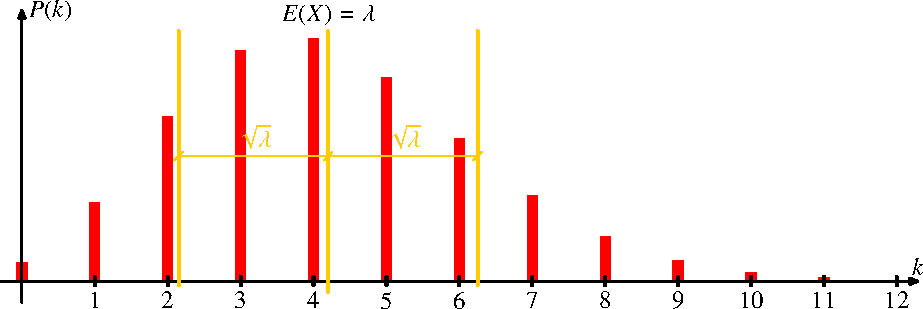
\includegraphics{images/exp-2.pdf}
\end{center}

\subsection{Sch"atzung des Parameters $\lambda$}
Der Parameter $\lambda$ ist der Erwartungswert einer Poisson-Verteilung,
er l"asst sich daher mit dem Mittelwert
\[
\hat\lambda(k_1,\dots,k_n)=\frac{k_1+\dots+k_n}n
\]
erwartungstreu sch"atzen.


\vfill
